\begin{comment}
\begin{figure*}[!t]
    \begin{minipage}[c]{0.28\textwidth}
            \centering
            \vspace{2pt}
            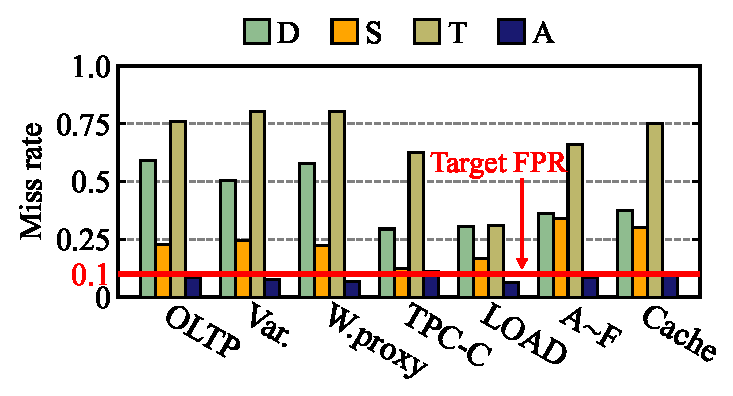
\includegraphics[width=\textwidth]{exp/miss_ratio/final-miss-ratio.eps}
            \vspace{-7pt}
   	        \caption{\FIXME{Miss ratio}} 
   	        \vspace{-10pt}
            \label{fig:miss-ratio}
    \end{minipage}
	\begin{minipage}[c]{0.71\textwidth}
        \begin{subfigure}[b]{0.64\textwidth}
            \centering
            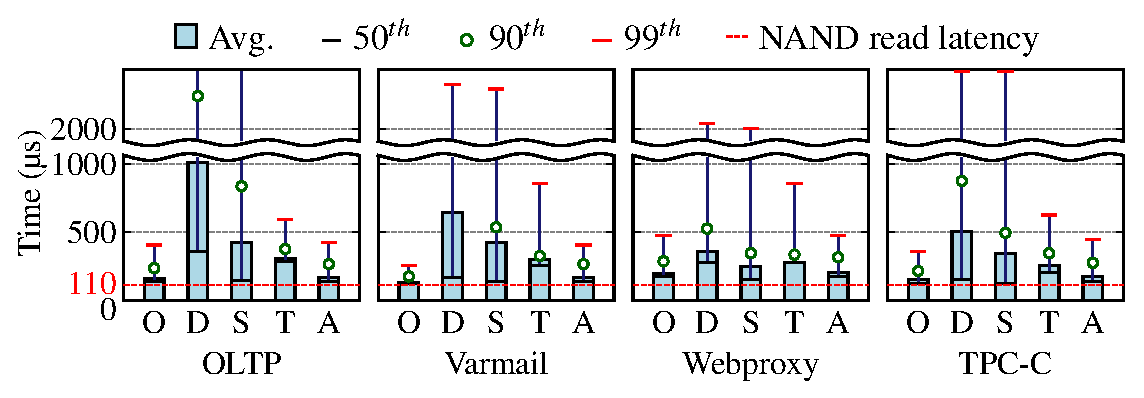
\includegraphics[width=\textwidth]{exp/filesystem/fs-latency.eps}
            \vspace{-10pt}
   	        \caption{\FIXME{Read latency}} 
            \label{fig:swap-latency}
        \end{subfigure}
        \begin{subfigure}[b]{0.345\textwidth}
            \centering
            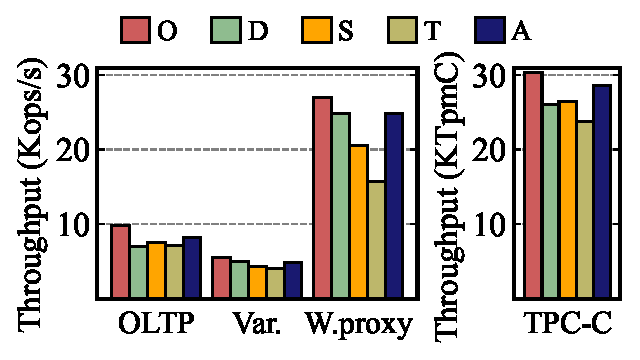
\includegraphics[width=\textwidth]{exp/filesystem/final-fs-throughput.eps}
            \vspace{0pt}
            \caption{Throughput} 
            \label{fig:swap-throughput}
        \end{subfigure}
        \vspace{-10pt}
	    \caption{Experimental results of Filebench and TPC-C}
	    \vspace{-10pt}
	    \label{fig:exp-fs}
	\end{minipage}
\end{figure*}
\end{comment}


\section{Experiments}
\label{sec:exp}
We show experimental results using realistic benchmarks,
%Since we already presented microscopic results in
%\SEC{sec:new-design}, we 
focusing on three performance aspects of \ours{}:
(\textit{i}) read latency, (\textit{ii}) I/O throughputs,
and (\textit{iii}) computation overheads.
%We focus on evaluating following three
%aspects of \ours{}: (\textit{i}) read latency, (\textit{ii}) I/O
%throughputs, and (\textit{iii}) impact of write optimization.

\begin{figure*}[t]
	\begin{minipage}[c]{0.71\textwidth}
        \begin{subfigure}[b]{0.64\textwidth}
            \centering
            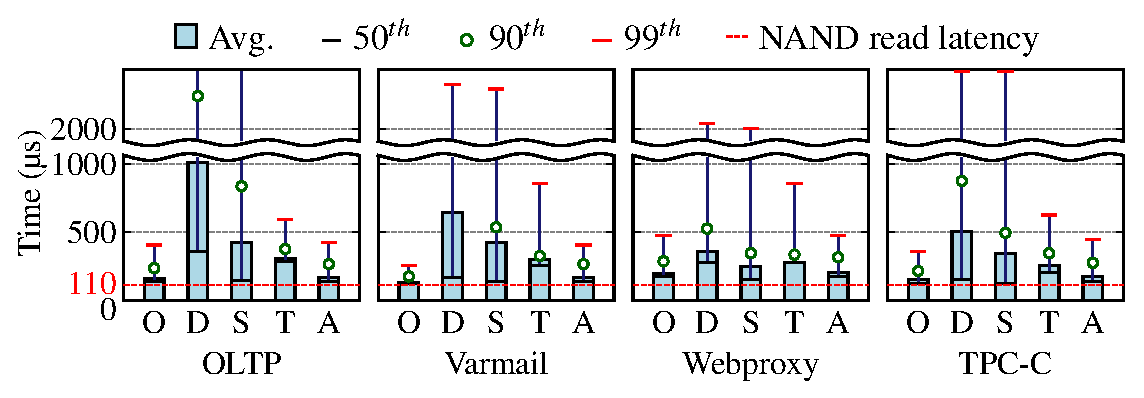
\includegraphics[width=\textwidth]{exp/filesystem/fs-latency.eps}
            \vspace{-10pt}
   	        \caption{Read latency}
            \label{fig:swap-latency}
        \end{subfigure}
        \begin{subfigure}[b]{0.345\textwidth}
            \centering
            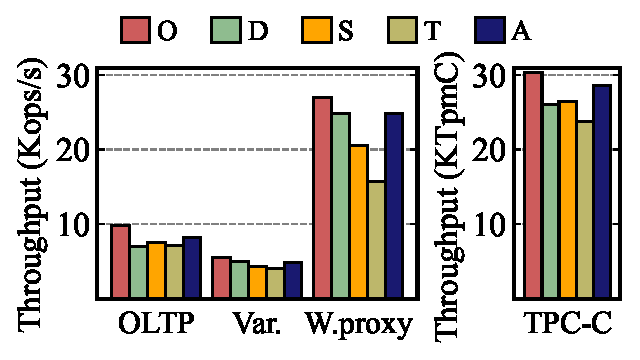
\includegraphics[width=\textwidth]{exp/filesystem/final-fs-throughput.eps}
            \vspace{-5pt}
            \caption{Throughput} 
            \label{fig:swap-throughput}
        \end{subfigure}
        \vspace{-7pt}
	    \caption{Experimental results of Filebench and TPC-C}
	    \vspace{-10pt}
	    \label{fig:exp-fs}
	\end{minipage}
    \begin{minipage}[c]{0.28\textwidth}
            \centering
            \vspace{0pt}
            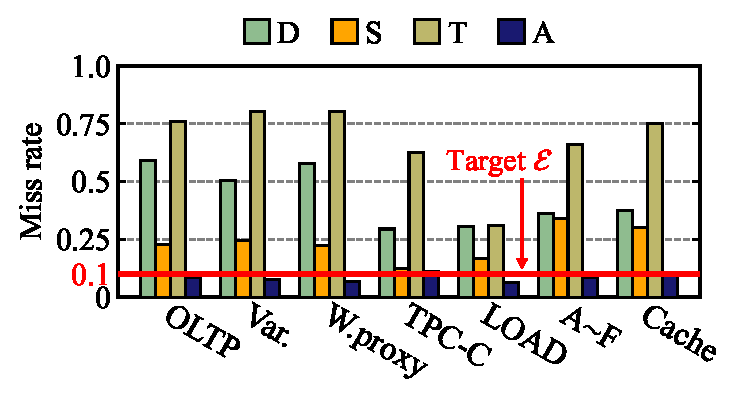
\includegraphics[width=\textwidth]{exp/miss_ratio/real-final-miss-ratio.eps}
            \vspace{-2pt}
   	        \caption{Miss rate}
            \vspace{-5pt}
            \label{fig:miss-ratio}
    \end{minipage}
    \vspace{-5pt}
\end{figure*}
%\vspace{-5pt}
\subsection{Experimental Setup}
\label{sec:exp:setup}

All experiments are conducted on a machine with Intel's i9 CPU (12
cores running at 4.6 GHz) and 4GB DRAM. We use an FPGA-based PCIe
Open-channel SSD employing custom flash cards that has 512GB capacity
and offers
2.4 GB/s read and 860 MB/s write throughputs.
The page size is 16KB,
and the number of pages per block is 128.  
We implement various translation policies on the x86 host like
ones~\cite{dm-zoned, ocssd} for ZNS and OCSSD. 
For fast evaluation, the SSD capacity is set to
64GB.  The over-provisioning space is 15\%.

Including \ours{}, we implement four popular policies, the optimal FTL (denoted
by \texttt{OPT})~\cite{flash-based-ssd
}, DFTL~\cite{dftl}, 
SFTL~\cite{sftl}, and TPFTL~\cite{tpftl}.  
\OPT{} maintains all the exact mapping entries in DRAM.
%A mapping entry size is
%40-bit under the assumption that the SSD capacity is larger than 32-TB.
%For a indexing table, 80-MB DRAM -- 0.125\% of SSD's capacity --
%is required. 
\OPT{} is infeasible in that it consumes lots of DRAM, when the SSD size is
huge.
%Note that 32-TB SSD needs 33-bit for pointing all 4-KB sectors in SSD, but
%33-bit does not align in byte-address.
%To index mapping entries, all policies except for \SECTOR{}
%use 24\% (19.2-MB) of DRAM that \SECTOR{} requires.
\DFTL{} keeps only popular entries in DRAM that are managed by LRU. \SFTL{} and
\TPFTL{} are variants of \DFTL{}.  \SFTL{} behaves as explained in
\SEC{sec:back:table}.  \TPFTL{} improves a cache hit rate by employing
two-level LRUs: one for indexing chunks (ICs) and the other for mapping entries
within chunks.  It also delta-encodes consecutive mapping entries.  The main
difference between  \SFTL{} and \TPFTL{} is a caching granularity. In
contrast to \SFTL{} that caches mapping entries belonging to the same 4KB IC,
\TPFTL{} caches popular mapping entries (\ie~<$x_i$, $y_i$>) to efficiently
use DRAM space only for hot entries.
%(\ie~indexing chunk in \SFTL{} and mapping entry in \TPFTL{}).
\OURS{} uses the balanced tree setup with three levels, as explained in
\SEC{sec:design:tree}, but it scales down the L0 size from 5.4GB to 332MB
as we use a smaller SSD (1TB vs 64GB).  A target FPR is set to 0.1.  All the
FTLs use the 1MB write-buffer (the memtable in the case of \ours{}).
For indexing, \texttt{OPT} uses 64MB DRAM (0.1\% of 64GB) and
the other FTLs use 18.6MB (29.1\% of \texttt{OPT}'s memory).
%assuming that the underlying SSD capacity is 16TB.
%\todo{(DRAM for mapping table)}


%\fixme{
We evaluate the FTLs under three representative systems that use SSDs as file,
swap, and cache storage, respectively.
%We evaluate the FTL techniques in three representative systems that use SSDs as
%their storage (\ie~file system, swap, and cache system).  
For file-system benchmarks, we use two Filebench~\cite{filebench} and
TPC-C~\cite{TPC-C} that run on EXT4.  For file-system
aging, we run Geriatrix~\cite{geriatrix}, a fragmentation tool, over EXT4
before running benchmarks. 
%After the aging, the SSD utilization is 49\%.  
To
emulate a use case of SSDs as swap storage, we run YCSB~\cite{ycsb} over Redis,
a popular in-memory KV store~\cite{redis}.  Finally, to evaluate performance
when SSDs are used for a cache service, we run CacheLib~\cite{cachelib}.
%We also use YCSB~\cite{ycsb} and CacheLib~\cite{cachelib} as swap
%and cache system benchmarks, respectively.  Filebench and TPC-C are run on EXT4
%as the default file system.}
%To emulate aged file systems, we run Geriatrix~\cite{geriatrix}, a
%fragmentation tool, over EXT4 before running benchmarks. After the
%aging, the SSD utilization is 49\%.  

\subsection{Experimental results}
%\JS{We refer to the miss ratios and WAFs of FTL techniques
%on benchmarks to explain their performances. 
%All of the miss ratios and WAFs are illustrated in \FIG{fig:miss-ratio} 
%and Table~\ref{tab:waf}, respectively.}
%\JS{In all figures of experimental results, \texttt{OPT}, \texttt{DFTL}, \texttt{SFTL}, \texttt{TPFTL}, and \texttt{APX-FTL}
%are abbreviated as `\texttt{O}', `\texttt{D}', `\texttt{S}', `\texttt{T}', and `\texttt{A}'.}

\begin{comment}
\begin{figure}[t]
\centering
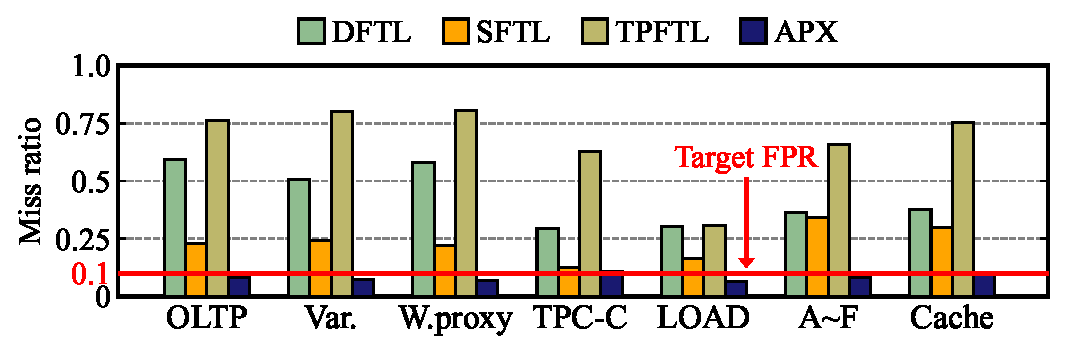
\includegraphics[width=0.93\linewidth]{exp/miss_ratio/new-miss-ratio.eps}
\vspace{-10pt}
\caption{\FIXME{Miss ratio}}
\vspace{-10pt}
\label{fig:miss-ratio}
\end{figure}
\end{comment}



\subsubsection{Results from File-system Benchmarks}
\label{sec:exp:fs}
%To evaluate \ours{} when it is used for file systems, we performs experiments
%using Filebench and TPC-C database benchmark.  
We choose three workloads from Filebench: \texttt{OLTP}, \texttt{Varmail}, and
\texttt{Webproxy}. The Filebench workloads have two phases, load and run.  In
the load phase, all workloads create files so that 77\% of the SSD is filled
with data. During the run phase, \texttt{Varmail} and \texttt{Webproxy} issue
8M and 4M operations over the created files, \texttt{OLTP} runs for 480
seconds.  In the case of TPC-C, we use PostgreSQL~\cite{postgresql} as RDBMS.
We create 220 warehouses before running TPC-C.  After creating the warehouses,
we run TPC-C for 10 minutes.

\begin{figure*}[t]
    %\vspace{0pt}
	\begin{minipage}[c]{0.622\textwidth}
        \begin{subfigure}[b]{0.45\textwidth}
            \centering
            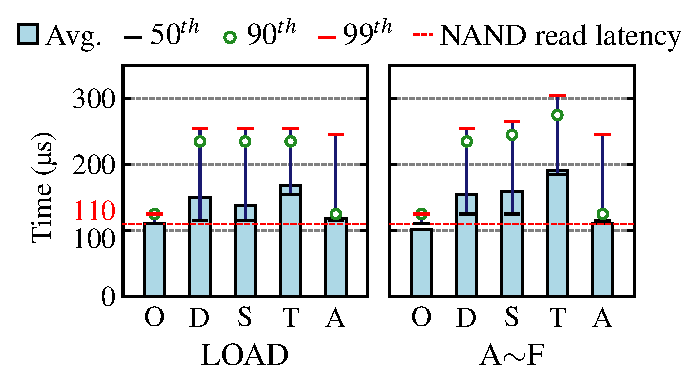
\includegraphics[width=\textwidth]{exp/swap/swap-latency.eps}
            \vspace{-13pt}
   	        \caption{Read latency}
            \label{fig:swap-latency}
        \end{subfigure}
        \begin{subfigure}[b]{0.51\textwidth}
            \centering
            \vspace{0pt}
            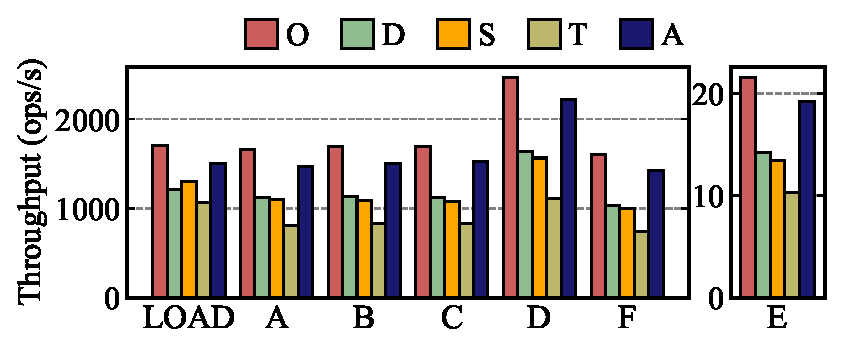
\includegraphics[width=\textwidth]{exp/swap/new_SWAP_throughput.eps}
            \vspace{-1pt}
            \caption{Throughput} 
            \label{fig:swap-throughput}
        \end{subfigure}
        \vspace{-10pt}
	    \caption{Experimental results of YCSB benchmark}
	    \label{fig:exp-swap}
	    \vspace{-15pt}
	\end{minipage}
	\begin{minipage}[c]{0.368\textwidth}
        \begin{subfigure}[b]{0.52\textwidth}
            \centering
            \vspace{8pt}
            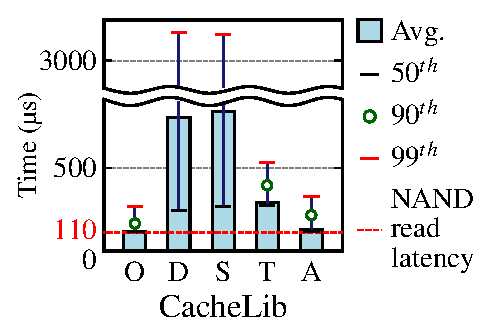
\includegraphics[width=\textwidth]{exp/cache/cache-latency.eps}
   	        \caption{Read latency}
            \label{fig:cache-latency}
        \end{subfigure}
        \hspace{5pt}
        \begin{subfigure}[b]{0.32\textwidth}
            \centering
            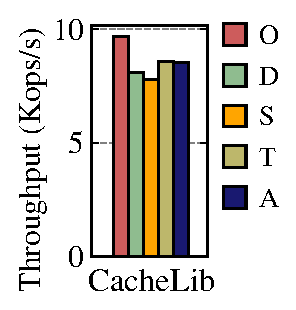
\includegraphics[width=\textwidth]{exp/cache/new_cache_th.eps}
            \vspace{-9pt}
            \caption{Throughput} 
            \label{fig:cache-throughput}
        \end{subfigure}
        \vspace{-10pt}
	    \caption{Experimental results of cache system}
	    \vspace{-15pt}
        \label{fig:expcache}
    \end{minipage}

\end{figure*}

\begin{comment}
\begin{figure}[t]
    \centering
    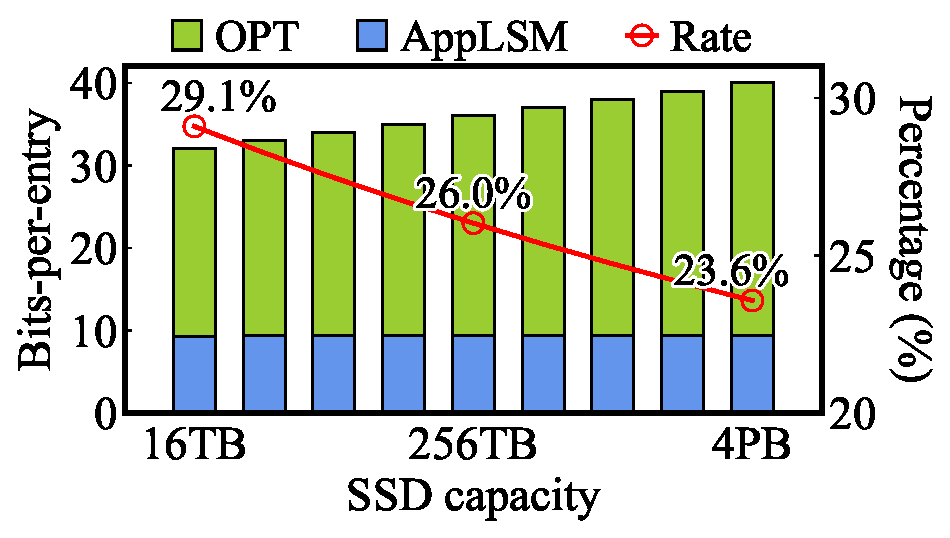
\includegraphics[width=0.28\textwidth]{figs/Figure_lsm_design/lsm_design/scale/plr-scale.eps}
    \caption{Scalability w/ SSD size}
    \label{fig:scalability}
\end{figure}
\end{comment}

\begin{comment}
\begin{figure}[t]
    %\vspace{0pt}
    \begin{subfigure}[b]{0.475\textwidth}
        \centering
        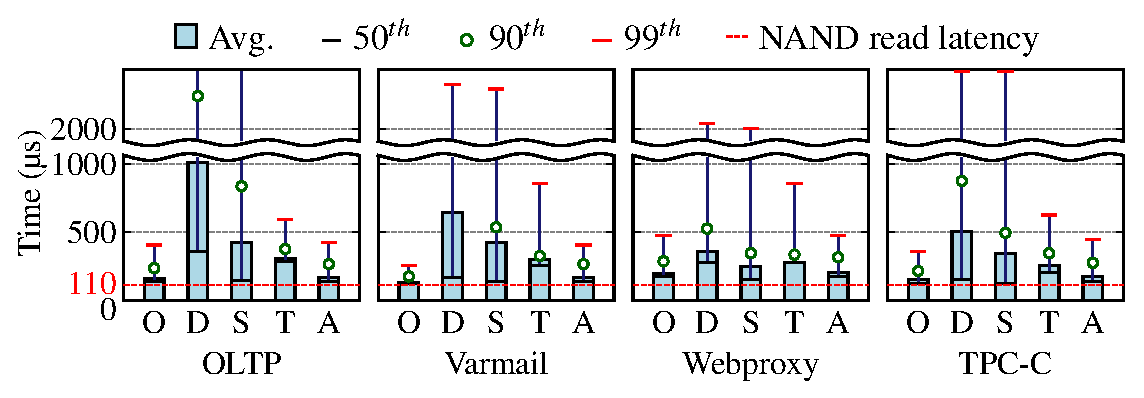
\includegraphics[width=\textwidth]{exp/filesystem/fs-latency.eps}
        \caption{Read latency}
        \label{fig:fs-latency}
        \vspace{5pt}
    \end{subfigure}
    \begin{subfigure}[b]{0.38\textwidth}
        \centering
        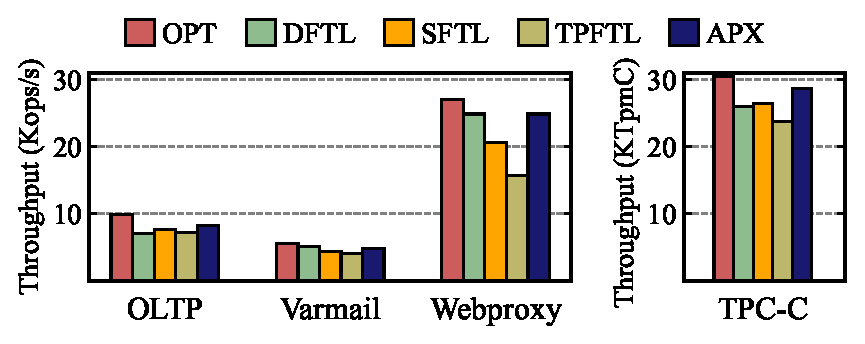
\includegraphics[width=\textwidth]{exp/filesystem/FS_throughput.eps}
        \caption{Throughput} 
        \label{fig:fs-throughput}
    \end{subfigure}
    \vspace{-10pt}
    \caption{Experimental results of Filebench and TPC-C}
    \label{fig:exp-fs}
    \vspace{-10pt}
\end{figure}
\end{comment}

\FIG{fig:exp-fs}(a) shows the average read latency, 
along with 50$^{th}$, 90$^{th}$, and 99$^{th}$ percentile latencies.
The red-dotted line at 110$\mu s$ indicates the
NAND read latency.  
Be advised that 
\texttt{OPT}, \texttt{DFTL}, \texttt{SFTL}, \texttt{TPFTL}, and \texttt{\ours{}}
are abbreviated as `\texttt{O}', `\texttt{D}', `\texttt{S}', `\texttt{T}', and `\texttt{A}', respectively, in figures.
For all the workloads, \OURS{} outperforms the demand-based
techniques, \DFTL{}, \SFTL{}, and \TPFTL{}; it achieves 67.1\%, 62\%, 30.8\%,
and 52.3\% shorter average read latency for \texttt{OLTP}, \texttt{Varmail},
\texttt{Webproxy}, and \texttt{TPC-C}.  All the demand-based FTLs suffer from
high cacahe miss rates (20\%$\sim$74.4\% on average; see \FIG{fig:miss-ratio}), showing longer
average latency.
%Especially, \texttt{DFTL} and \texttt{SFTL} show
%long-tail latency since they have high dirty eviction rates.  
On the other hand, \OURS{} exhibits read latency very close to that of
\texttt{OPT} thanks to its low error rates (6.8\%$\sim$10.8\%). For 
some workloads, \OURS{} exhibits lower error rates (6.8\%$\sim$8.2\%) than
expected 10\% as shown in \FIG{fig:miss-ratio}.  
%Our close examination reveals that 
It is owing to the impact of LBA sorting.  Since \ours{} sorts logical
blocks by their LBAs, consecutive blocks are likely to be stored in the same 16KB
page.  This facilitates prefetching of soon-to-be read blocks.
%For some workloads that have spatial locality, \ours{} can prefetch
%soon-to-be read blocks.  
%This reduces the FPR of \OURS{} to lower than expected.
%1. Read is faster
%2. impact of write on application-perceived throughput is low owing to write buffering
%3. varmail -> fsynca -> application-perceived write latency is worse than others. 
\begin{comment}
\begin{figure*}[t]
    %\vspace{0pt}
	\begin{minipage}[c]{0.622\textwidth}
        \begin{subfigure}[b]{0.45\textwidth}
            \centering
            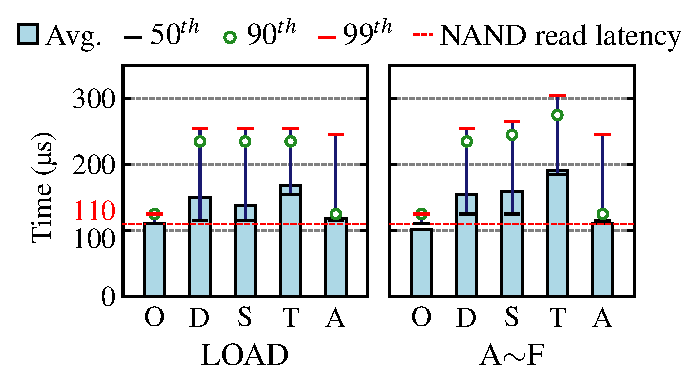
\includegraphics[width=\textwidth]{exp/swap/swap-latency.eps}
            \vspace{-13pt}
   	        \caption{\FIXME{Read latency}} 
            \label{fig:swap-latency}
        \end{subfigure}
        \begin{subfigure}[b]{0.51\textwidth}
            \centering
            \vspace{0pt}
            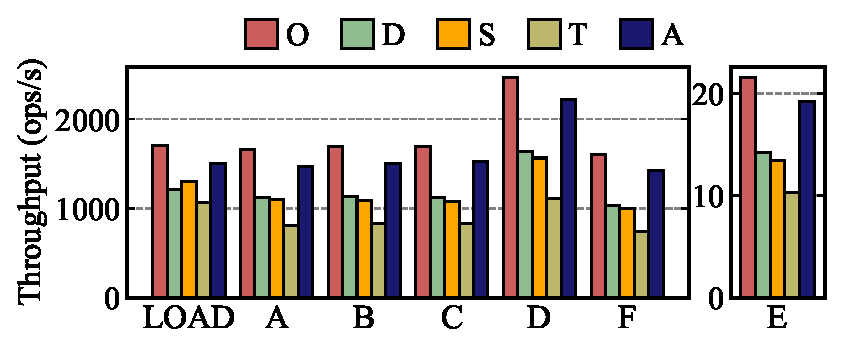
\includegraphics[width=\textwidth]{exp/swap/new_SWAP_throughput.eps}
            \vspace{-1pt}
            \caption{Throughput} 
            \label{fig:swap-throughput}
        \end{subfigure}
        \vspace{-12pt}
	    \caption{Experimental results of YCSB benchmark}
	    \label{fig:exp-swap}
	    \vspace{-10pt}
	\end{minipage}
	\begin{minipage}[c]{0.368\textwidth}
        \begin{subfigure}[b]{0.52\textwidth}
            \centering
            \vspace{8pt}
            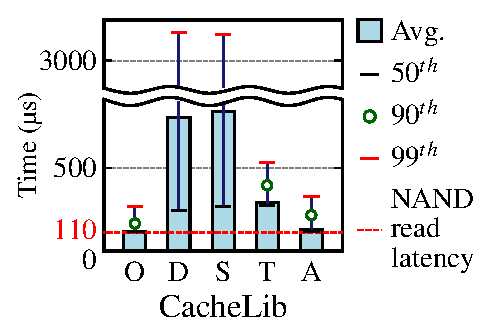
\includegraphics[width=\textwidth]{exp/cache/cache-latency.eps}
   	        \caption{\FIXME{Read latency}} 
            \label{fig:cache-latency}
        \end{subfigure}
        \hspace{5pt}
        \begin{subfigure}[b]{0.32\textwidth}
            \centering
            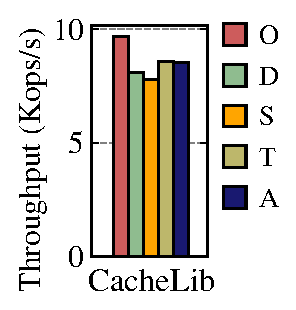
\includegraphics[width=\textwidth]{exp/cache/new_cache_th.eps}
            \vspace{-9pt}
            \caption{Throughput} 
            \label{fig:cache-throughput}
        \end{subfigure}
        \vspace{-13pt}
	    \caption{Experimental results of cache system}
	    \vspace{-10pt}
        \label{fig:exp-cache}
    \end{minipage}
\end{figure*}
\end{comment}

\setlength{\tabcolsep}{0.33em}
{\renewcommand{\arraystretch}{0.6}
\begin{table}[b]
    \footnotesize
    \centering
    \vspace{-5pt}
    \caption{A comparison of WAFs of FTLs}
    \begin{tabular}{|c||c|c|c|c|c|c|}
        \hline
            Benchmark       &  OLTP & Var. & W.proxy   & TPCC & YCSB    & CacheLib\\ 
                                (R:W ratio)    &  (1:1.13) & (1:2.7)   &(1:0.7)   & (1:2.45)   &(1:1)       & (1:0.7)\\ \hline\hline
            \texttt{OPT}	        & 3.90      & 4.22        & 2.33      &3.51   &1.48   &1.60\\ \hline
            \texttt{DFTL}	        & 6.02      & 4.93        & 2.51      &4.35   &1.51   &6.61\\ \hline
            \texttt{SFTL}	        & 4.56      & 4.71        & 2.50      &3.87   &1.51   &6.56\\ \hline
            \texttt{TPFTL}	        & 4.10      & 4.58        & 2.50      &3.75   &1.49   &1.86\\ \hline
            \texttt{\ours{}}	    & 5.11      & 5.35        & 3.01      &4.08   &2.94   &4.32\\ \hline
            %\texttt{APX-unopt}	    & 6.17      & 6.5        & 4.06      &5.19   &3.95   &5.62\\ \hline
            %R:W	                    & 1:1.13    & 1:2.7       & 1:0.7     &1:2.45 &1:1    &1:0.7\\ \hline
    \end{tabular}
    %\caption{WAF and R:W ratio of benchmarks, \texttt{APX-unopt} is \texttt{\ours{}} without WAF optimization in \SEC{sec:impl}. \texttt{YCSB} shows the average WAFs and R:W ratio.}
    %\caption{WAF of FTLs, the (R:W) ratios are below the benchmarks,\texttt{YCSB} shows the average WAF of FTLs and R:W ratio.}
    %\vspace{-20pt}
    \label{tab:waf}
    \vspace{-5pt}
\end{table}
}

\FIG{fig:exp-fs}(b) shows the throughput of the four benchmarks.
Even though \texttt{\ours{}} has higher WAFs (see Table~\ref{tab:waf}), \OURS{}
shows similar or even higher throughput than the demand-based FTLs.  
First, the throughput drop by slow writes is offset by the high read
throughput of \ours{}.  Second, thanks to write buffering, the relatively
slow write throughput of \ours{} does not seriously affects
application-perceived performance.  For example, \texttt{OLTP} spawns three
threads to emulate database workload: two for writing logs and DB data; and one
for reading DB data.  The two writing threads issue requests asynchronously,
buffering data in the page cache. Therefore, application-perceived delays are
not significant. On the other hand, in the case of \texttt{Varmail} that frequently
invokes \texttt{fsync()}s, \ours{} provides slightly lower throughput
than \DFTL{}. \texttt{fsync()} is a synchronous operation, so applications 
must wait until it is complete. This results in a non-trivial throughput drop.
%Note that \texttt{SFTL} has lower miss ratios than \texttt{DFTL}, 
%but it shows lower throughputs, owing to decompression overheads.

%For \texttt{TPC-C}, \OURS{} shows 8\%$\sim$20\% higher throughput over demand-based policies 
%with a similar reason in \texttt{OLTP}.

\begin{comment}
\fixme{
%in spite of its high WAF (see Table~\ref{tab:waf}).
\texttt{OLTP} has three threads to emulate the OLTP database workload:
two for writing log and DB data, respectively, and one for reading DB data.
%which are two threads for writing (log and database data) and one for reading.
Since the two writing threads issue requests asynchronously, 
the write overhead less affects \texttt{OLTP} throughput.
Thus, \OURS{} outperforms 8\%$\sim$16\% higher comparing demand-based FTLs.
\texttt{Varmail} and \texttt{Webproxy} does not issue their write asynchronously.
The throughput at the two workloads tends to follow policies' WAF, miss ratio (see \FIG{fig:miss-rate})
and workloads' read-write ratio (see Table~\ref{tab:waf}).
Although \texttt{Varmail} has more write requests and \OURS{} has high WAF,
\OURS{} shows comparable performance since other policies suffer from cache-miss
that affects read and write performance.
In \texttt{Webproxy}, \OURS{} shows similar or higher performance in that
\texttt{Webproxy} has more read requests.
Note that \texttt{SFTL} has lower miss rates than \texttt{DFTL}, 
but it shows lower throughput owing to its decompress overhead.
For \texttt{TPC-C}, \OURS{} shows 8\%$\sim$20\% higher throughput over demand-based policies 
with a similar reason in \texttt{OLTP}.
}
\end{comment}



\subsubsection{Results from Swap Benchmarks}

We then evaluate the FTLs when they are used for
swap storage.  We use YCSB as a benchmark and run it on Redis~\cite{redis}.  We
populate 20M KV pairs during the load phase.  Each KV pair is 1KB in size.
After loading KV pairs, we run 6 workloads (\ie~\texttt{YCSB-A$\sim$F}) for 20 minutes
per workload.  We use the default parameters of YCSB.

% write buffer hit

% high waf but less impact

% read requests are issued one by one every 200~300 us. 
% 99% tail -DFTL, SFTL, TPFTL has short 99% tail latency (250-300us at 99th)
% than file-system (2ms at 99th);

\begin{comment}
\begin{figure}[t]
\centering
%\includegraphics[height=5.3cm]{test.eps}
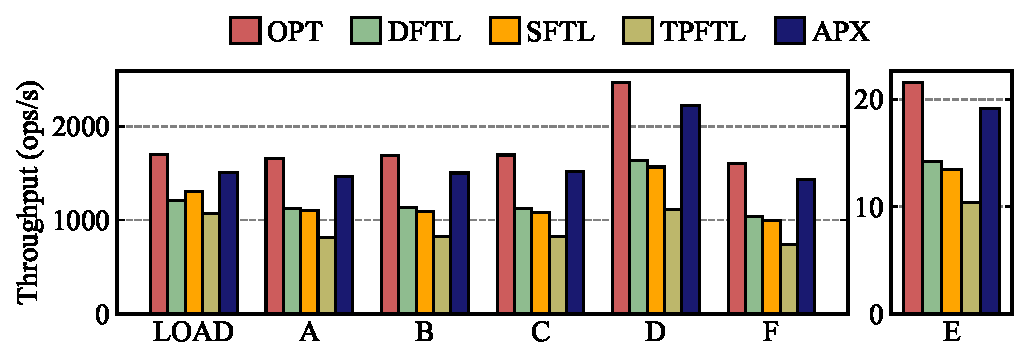
\includegraphics[width=0.93\linewidth]{exp/swap/SWAP_throughput.eps}
%\vspace{-3pt}
\caption{\FIXME{Throughput of YCSB}}
\label{fig:swap-throughput}
\end{figure}

\end{comment}

\FIG{fig:exp-swap} compares the read latency and throughput of the
FTLs (it displays only \texttt{LOAD} and \texttt{YCSB-D} since \texttt{A$\sim$F} show similar 
results).
%\JS{All FTLs show almost the same read latency trends in YCSB A$\sim$F, 
%thus we illustrate the representative result in \FIG{fig:exp-swap}(a).}
%Similar to the results from the file-system benchmarks, 
\texttt{\ours{}} exhibits
shorter read latency than the demand-based FTLs.
%, in terms of average,
%50$^{th}$, 90$^{th}$, and 99$^{th}$ percentiles.  
One of the noticeable
observations is that the demand-based FTLs less suffer from long tails,
exhibiting
%In the swap benchmark, they exhibit 
250$\mu$s$\sim$305$\mu$s latency at the
99$^{th}$ percentile.  This is much shorter than the 99$^{th}$ latency of the
file-system benchmarks that reaches up to 3.3$m$s.  This is due to the
unique behavior of the Linux swap system.  Compared to the file-system
benchmarks that heavily issue a large number of I/Os, the Linux swap
system sporadically issues read requests at intervals of 200$\mu$s$\sim$300$\mu$s.
Under the file-system benchmarks, upon a mapping cache miss, subsequent reads
are delayed until the missed request is served, which results in long tails.
In the swap system, such delays occasionally happen, and thus the
demand-based FTLs exhibit better read tails.  \texttt{\ours{}} performs better than the
demand-based FTLs, but shows longer tails than \texttt{OPT} owing to
false positive results of BFs that requires up to two extra reads.

%Another interesting observation is that 
%\texttt{OPT} and \ours{} exhibit
%shorter read latency than NAND read latency. We observe that the swap system
%often reads data which have just written before. The write buffer 
%hit ratio is about 15\%$\sim$17\%. The demand-based FTLs also take the
%same benefit, but because of high miss ratios, they
%show longer latency than NAND latency.
%their average read latencies are
%much longer than NAND read latency.

\FIG{fig:exp-swap}(b) compares the throughput of the FTLs.  In spite of
having higher WAFs than the other FTLs, \texttt{\ours{}} exhibits fairly good
throughputs, outperforming the demand-based ones.  Similar to the \texttt{OLTP} workload
in \SEC{sec:exp:fs}, the Linux swap system performs swap-out operations in background
to hide the long latency of flushing out dirty pages to the storage. As a
result, the negative impact of higher WAFs of \texttt{\ours{}} is negligible in the swap
system. On the other hand, the fast read latency of \texttt{\ours{}} directly benefits
the YCSB's performance. As shown in \FIG{fig:exp-swap}(b), \texttt{\ours{}} achieves
the throughputs close to that of \texttt{OPT}.

\begin{comment}
\fixme{
\FIG{fig:swap-latency} and \FIG{fig:swap-throughput} show the read latency and
throughput results, respectively.  Swap issues requests at intervals of
200$\sim$300 $\mu s$ which is larger than read I/O time in the NAND flash.
Thus, the latency results show each read request latency without queuing delay.
Even if the SSD is initial states, all six workloads have a weak locality in
their requests.  \OURS{} shows almost the same average latency performance as
\SECTOR{} thanks to its approximate indexing algorithms.  About 15\%$\sim$17\%
of read requests do not read NAND since they are hit at the write-buffer for
all FTLs, thus \OURS{} and \SECTOR{} have lower average latency than the NAND
read latency.  However, the other FTLs have the delayed average latency in that
they suffer from high miss rates (15\%$\sim$75\%).  Although \OURS{} cannot
guarantee the $99\%$ long-tail latency owing to the target FPR (\ie~0.1), it
has shorter long-tail latency than the other demand-based techniques.  The
notable thing is that \OURS{} outperforms other demand-based policies in
throughput (see \FIG{fig:swap-throughput}).  The workloads issues read and
write at a similar ratio.  \OURS{} has quite higher WAFs (1.34$\sim$1.68
higher, see Table~\ref{tab:waf}) than other policies.  Despite it, \OURS{}
shows much higher throughput (30\%$\sim$92\% better) compared with demand-based
policies.  Linux kernel writes infrequently accessed data to its swap area.
The writing data from page cache to storage is done in background.  However,
when an application reads data in the swap area, it should directly read the
data from storage.  Therefore, the swap performance highly depends on storage
read performance.  As a result, \OURS{} has the best performance except for
\SECTOR{} in the swap scenario.  Especially in workload E range-query most
workload, \OURS{} shows the highest gap compared with demand-based policies.
}
\end{comment}

\subsubsection{Results from Cache Benchmarks}

We evaluate the FTLs when they are used as cache
storage. We use CacheLib, an SSD-based cache system platform from
Facebook~\cite{cachelib}. We use the \texttt{graph\_cache\_leader} workload for evaluation.
%to evaluate the performance.  
CacheLib is based on hashing like many other cache
systems~\cite{bluecache, kangaroo}.  Thus, it mostly issues random I/Os while
serving client requests.  We run 72M operations over 41M KV pairs. 
%CacheLib
%is a read-intensive workload; reads account for 59\% of the total
%requests.

\FIG{fig:cache-latency}(a) and \FIG{fig:cache-throughput}(b) show read latency and
throughput, respectively.  As expected, the demand-based FTLs severely suffer
from high miss rates because of random I/O patterns with weak locality.
\texttt{\ours{}} is less affected by such unique behaviors of CacheLib, thereby
exhibiting fairly good read latency comparable to \texttt{OPT}.  
\texttt{DFTL} and \texttt{SFTL} also
suffer from the highest WAFs among all the FTLs evaluated.  CacheLib issues a
large number of random writes to the SSD.  
Unlike \DFTL{} and \SFTL{}, 
\TPFTL{} writes many dirty entries to the flash in a batch manner on cache evictions.
Thus, \TPFTL{} shows a fairly low write overhead. 
\texttt{\ours{}} is based on the LSM-tree
which performs buffered writes in an append-only manner.
Thus, it also takes advantage of batch-writing.
\begin{comment}
\fixme{When they evict dirty entries, they
have to perform costly read-modify-write (RMW) operations that read in a
flash-resident IC, merges it with dirty entries to evict, and writes it back to
the flash. \TPFTL{} avoids costly RMWs by batch-writing only dirty
entries to the flash.
\texttt{\ours{}} is based on the LSM-tree, so it never causes
costly RMWs as up-to-date data are appended to the tree.}
\end{comment}
Consequently, \texttt{\ours{}} has low WAFs (see Table~\ref{tab:waf}),
showing similar or higher throughput than the demand-based FTLs.

%\subsubsection{\JS{Results of FP- and PLR-based indexing overhead}}
\subsubsection{Analysis of Indexing Overheads}
Finally, we measure the lookup time and rebuilding time of 
the FP- and PLR-based indexing on the two CPUs,
Intel i9-10920X and ARM Cortex-A53, which present high-end and 
embedded CPUs, respectively.
To assume the worst-case scenario, 
we run a micro-benchmark that reads data of 10GB randomly.
The FP-based indexing takes 0.2$\mu$s and 0.55$\mu$s on
Intel's CPU and ARM CPU, respectively.
The PLR-based indexing requires 0.25$\mu$s and 0.91$\mu$s 
on the two CPUs.
Typical NAND read latency is 100$\sim$120$\mu$s, so 
these lookup overheads are negligible. 
This implies that the FP- and PLR-based indexing are lightweight 
to run in an SSD with wimpy CPUs.

To evaluate the rebuilding time of approximate indices, 
we execute a benchmark that writes data of 10GB randomly.
The FP-based indexing needs 0.36s and 0.9s on Intel and ARM CPUs,
while the PLR-based indexing takes 0.64s and 6.8s, respectively.
PLR is more time-consuming than FP,
but in comparison with compaction I/O time for 10GB writes, 15.7
seconds, rebuilding times are negligible and 
are short enough to completely overlap with compaction I/Os.


\begin{comment}
\fixme{
\textbf{Cache system benchmark:}
CacheLib is an SSD-based cache system platform from Facebook.
We use graph\_cache\_leader workload that evaluates SSDs performance.
CacheLib is based on a hash algorithm like many other cache systems~\cite{bluecache, kangaroo}.
Thus, its request pattern has almost random.
We run 72M operations over 41M key-value pairs.
The number of read operations is more than write operations.
}

\fixme{
\FIG{fig:cache-result}(a) and \FIG{fig:cache-result}(b) show the results of read latency and
throughput, respectively.
As the cache engine is based on a hash algorithm, the demand-based FTLs suffer from high miss ratios. 
Since \ours{} is less affected by system's behavior on read performance,
it has good read latency. 
Unlikely any other systems, \texttt{DFTL} and \texttt{SFTL} show the highest WAFs among FTL techniques since 
the write requests have almost random patterns.
The random writes make many dirty evictions that need costly RMW operations in demand-based techniques.
\texttt{TPFTL} avoid RMWs by batch-writing dirty mapping entries, 
but \texttt{DFTL} and \texttt{SFTL} cannot avoid them since
their large size of cache entry (\ie~indexing chunk granularity) makes the number of batch-written cache entries fewer.
\ours{} uses batch-write for write requests to avoid RMW overhead by LSM-tree buffered write, 
but it shows higher WAF than \texttt{TPFTL} by its compaction overhead.
As a result, \OURS{} has the close throughput with \texttt{TPFTL} and better performance 
than \texttt{DFTL} and \texttt{SFTL} (see \FIG{fig:cache-result}(b)).
}
\end{comment}

\begin{comment}
\begin{figure}[t]
\centering
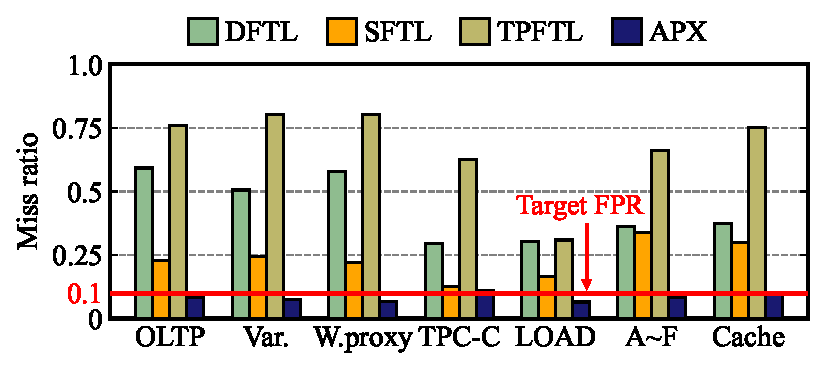
\includegraphics[width=0.84\linewidth]{exp/miss_ratio/miss-ratio.eps}
%\vspace{-3pt}
\caption{\FIXME{Miss ratio}}
\label{fig:miss-rate}
\end{figure}
\end{comment}

\begin{comment}
\textbf{Filebench:} 
To evaluate \OURS{} under realistic workloads, we perform experiments using
three workloads from Filebench: \textsf{OLTP}, \textsf{Varmail},
and \textsf{Webproxy} in \FIG{fig:filebench-results}. We use default parameters from
Filebench.
At the load phase, all workloads create files 
so that 87\% of SSD is filled with data.
During the run phase, \textsf{Varmail} and \textsf{Webproxy} 
issue 8M and 4M
operations over the created files. \textsf{OLTP} runs for 480 seconds.  

{\FIG{fig:filebench-results}(a)} shows the CDF of read latency.  For all 
Filebench workloads, \OURS{} outperforms the demand-based translation
techniques; it achieves 51\%, 75\%, and 52\% shorter average read latency
on \textsf{OLTP}, \textsf{Varmail}, and \textsf{Webproxy}.
\OURS{} exhibits read latency very close to that of \SECTOR{},
which is rather unexpected at first glance.
Close examination reveals that it is owing to the impact of LBA sorting. 
Although the storage space is severely fragmented, EXT4 attempts to
allocate neighboring LBAs to the same file. Since \OURS{} sorts logical blocks
by their LBAs, data from the same file is likely to be stored in the same 16-KB
page. The Filebench workloads tend to read the entire file data at once.
Since four logically consecutive 4-KB blocks are packed into the same NAND
page, \OURS{} can prefetch soon-to-be-read blocks. This reduces the FPR of \OURS{} to 0.05.

\FIG{fig:filebench-results}(b) shows the
throughput of the three benchmarks.  
Overall, the WAF is a major factor that decides overall I/O throughput. This is
because Filebench induces more writes than reads, which involve costly GC
or compaction (see Table~\ref{tab:waf}). 
For \textsf{OLTP}, \OURS{} exhibits the
best performance.  This is due to the relatively lower WAF of \OURS{} in
\textsf{OLTP}.  \textsf{OLTP} preallocates many log files (roughly 10-MB each)
and repeatedly overwrites log records over them.  As explained before, EXT4
tries to allocate neighboring LBAs to the same log file. On the \OURS{} side,
logical blocks from the same log file are likely to be stored in the same NAND
block.  Log data are frequently overwritten over user data. Thus, NAND
blocks containing log data become invalid soon, which in turn reduces page
copies during compaction.  In the other techniques, log data and other data are
mixed up in the same NAND flash. As a result of this,
they suffer from high GC costs.
\OURS{} also achieves I/O throughput
comparable to \SECTOR{}. 
Similar to \textsf{OLTP},
\textsf{Varmail} is a fsync-intensive workload that writes many
metadata to a preallocated journal.  Unlike \textsf{OLTP} and \textsf{Varmail},
\textsf{Webproxy} appends new data to many files,
allocating new LBAs far away from LBAs previously allocated to the files.
\OURS{} cannot benefit from LBA sorting; instead, owing to high compaction overhead, it
shows 19\% lower throughput than \DFTL{}.
\end{comment}



\begin{comment}
\textbf{Impact of WAF optimizations:}
We compare the WAFs between write-optimized \ours{} (\OURS{}) and 
unoptimized \ours{} (\texttt{APX-unopt}) in Table~\ref{tab:waf}. 
%The results show that 
As mentioned in \SEC{sec:impl}, the actual memory footprint of PLR models
is much lower than its worst-case memory usage.
We observe that 18$\sim$65\% leftover memory is available,
which can be assigned as indirection pointers for BF indices.
As a result, \texttt{\ours{}} has 21\% lower WAF than 
\texttt{APX-unopt}, on average. 
\end{comment}

\begin{comment}
\begin{figure*}[t]
\centering
\subfloat[Hit ratio]{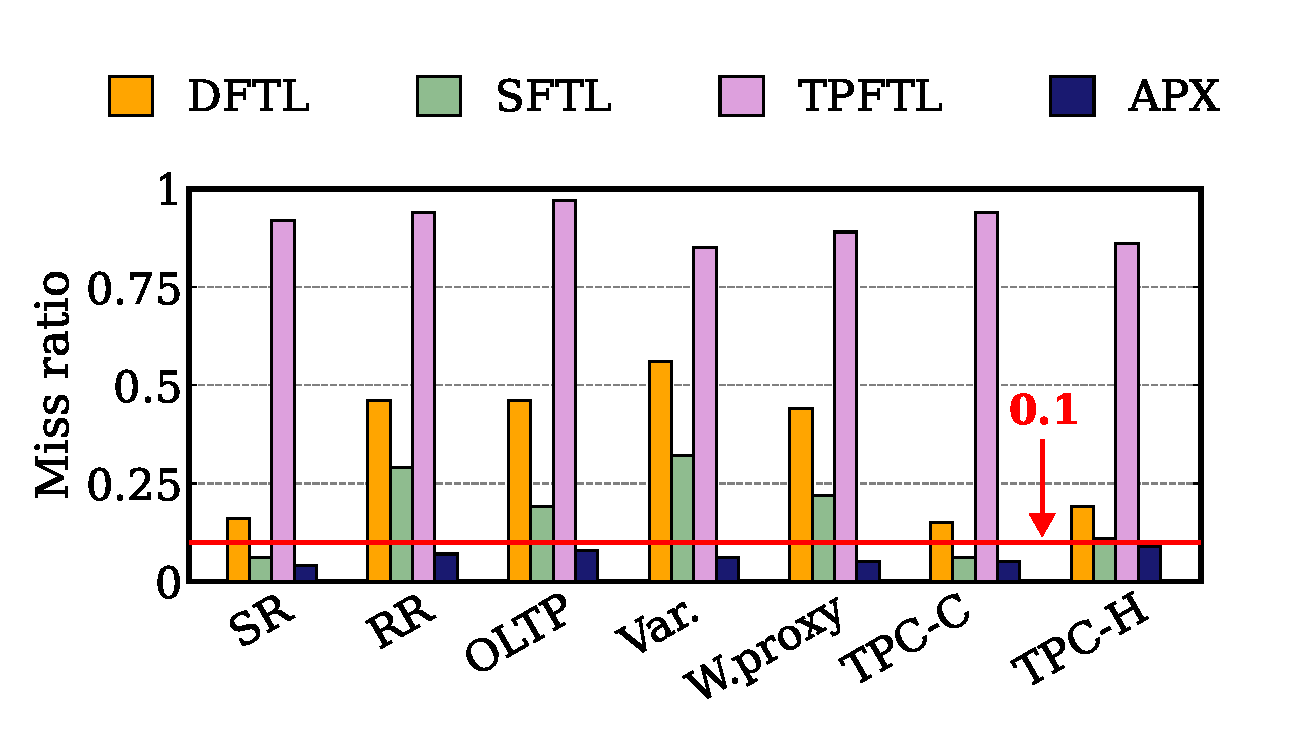
\includegraphics[height=3.6cm]{exp/miss_ratio/miss_ratio.eps}}
\subfloat[Throughput]{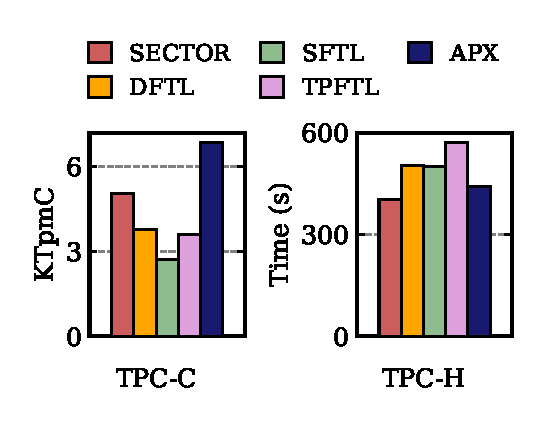
\includegraphics[height=3.8cm]{exp/tpc/TPC_run_throughput.eps}}
\hspace{5pt}
\subfloat[Latency]{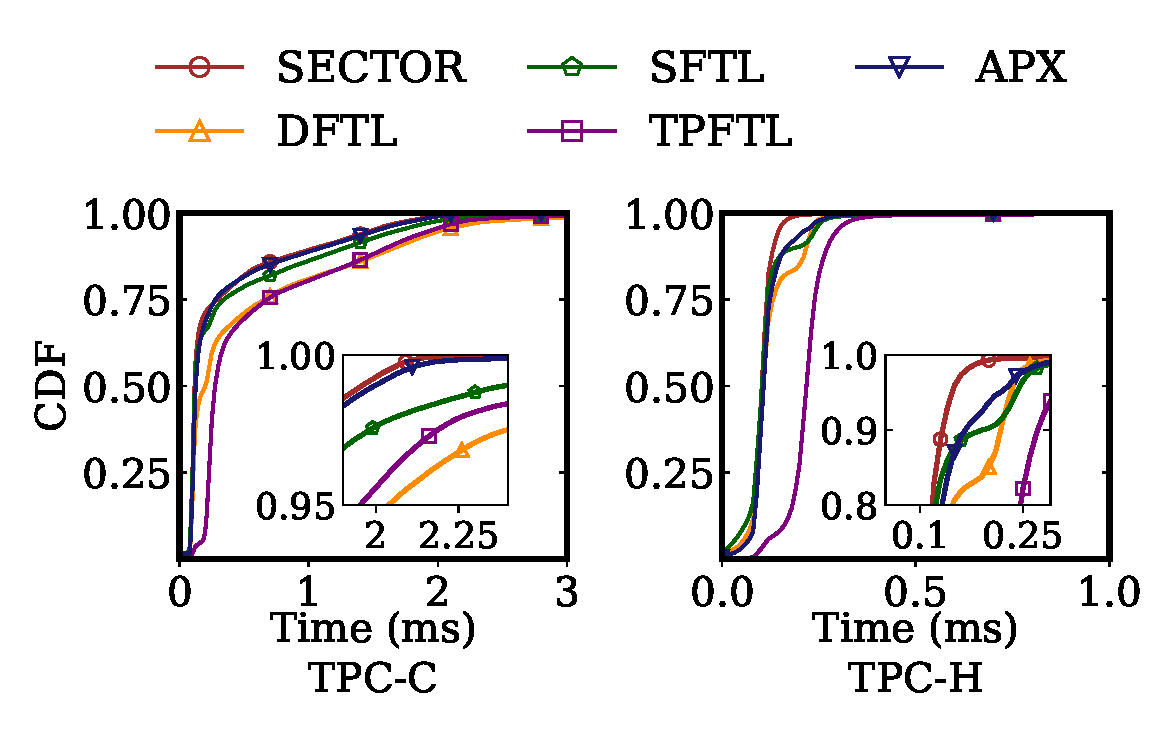
\includegraphics[height=3.7cm]{exp/tpc/TPC_t_latency.eps}}
\caption{
	\revise{Results of TPC}
}
\label{fig:filebench-result}
\end{figure*}
\end{comment}



\begin{comment}
\begin{figure}[t]
\centering
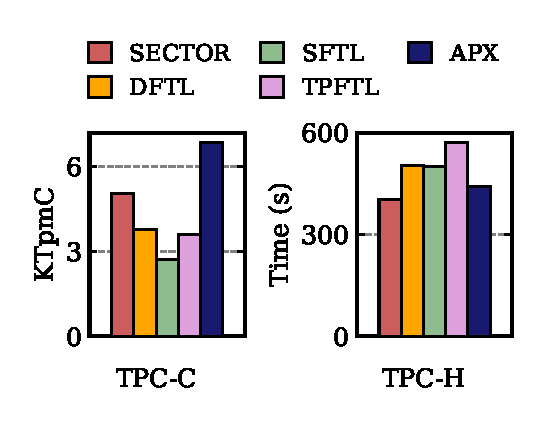
\includegraphics[width=7.7cm]{exp/tpc/TPC_run_throughput.eps}
\vspace{-10pt}
\caption{Throughput of database benchmarks}
\label{fig:db-throughput}
\end{figure}

\begin{figure}[t]
\centering
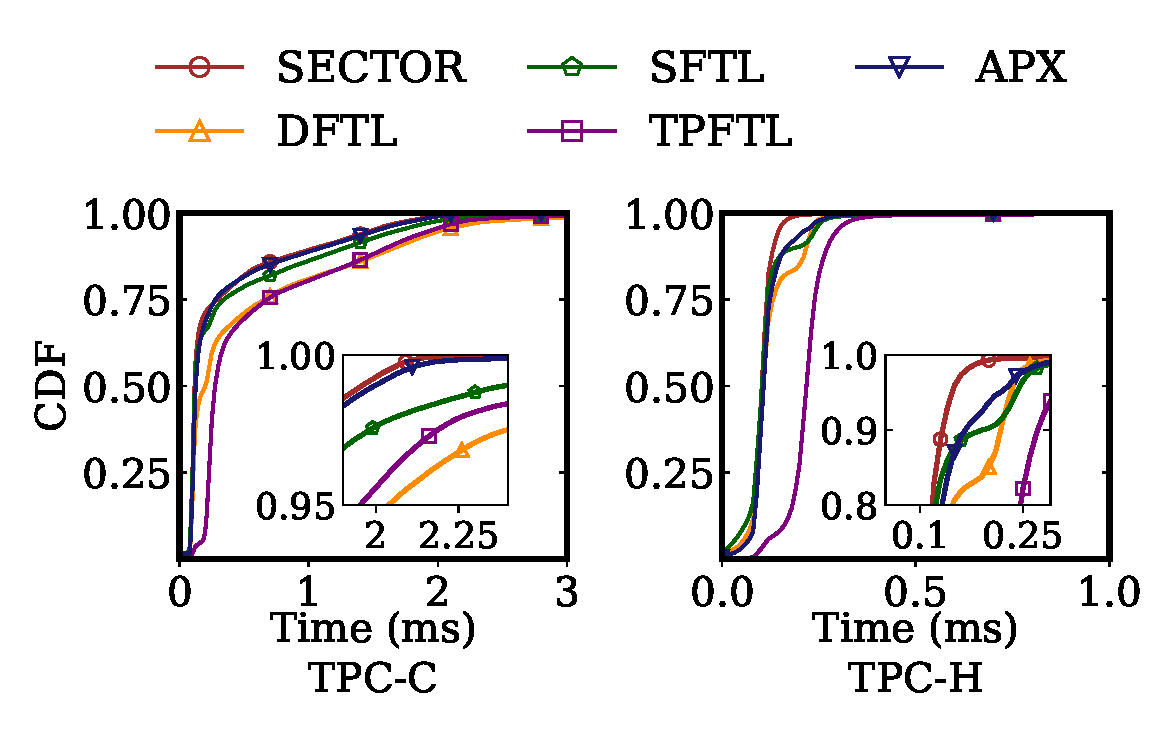
\includegraphics[width=7.7cm]{exp/tpc/TPC_t_latency.eps}
\vspace{-10pt}
\caption{CDF of read latency of database benchmarks}
\label{fig:db-latency}
\end{figure}
\end{comment}

\begin{comment}

{\renewcommand{\arraystretch}{0.9}
\begin{table}[t]
	\small
	\centering
	\begin{tabular}{|c|c|c|c|c|c|c}
		\hline
		    \begin{comment}
			Syscalls    & \textbf{\ours{}}     & \textbf{EXT4} \\ \hline \hline
			~\texttt{mkdir}       & SET(MO)             & W(BB + IB + I + DE)\\
			~\texttt{rmdir}       & DELETE(MO)          & W(BB + IB + DE)\\
			~\texttt{creat}       & SET(MO)             & W(IB + I + DE)\\
			~\texttt{unlink}      & DELETE(MO + DO)     & W(BB + IB + DE)\\
			~\texttt{setattr}     & SET(MO)             & W(I)\\
			~\texttt{write}       & SET(DO)             & W(BB + D)\\ \hline
			~\texttt{open}        & GET(MO)             & R(I)\\
			~\texttt{lookup}      & GET(MO)             & R(DE + I)\\
			~\texttt{read}        & GET(DO)             & R(D)\\
			~\texttt{readdir}     & ITERATE(MO)         & R(DE + I)\\ \hline
			
			~\bold{FTL}             & \bold{OLTP}     & \bold{Varmail}  & \bold{Webproxy}   & \bold{Webserver} \\ \hline \hline
            ~\texttt{PAGE}	        & 4.60            & 4.85            & 4.27              & 2.98\\ \hline
            ~\texttt{APX-FTL}	    & 3.75            & 5.31            & 5.55              & 5.61\\ \hline
            ~\texttt{Others-min}	& 5.43            & 6.80            & 4.62              & 4.68\\ \hline
            \end{comment}
    \end{tabular}
	\caption{Results of WAF in filebench, Others-min is the best WAF among \texttt{COARSE, FINE, SFTL, TPFTL}}
	\vspace{-5pt}
	\label{tab:filebench-waf}
\end{table}
}
\end{comment}


\begin{comment}
\textbf{Fio:} 
To understand the performance characteristics of \OURS{} under basic I/O
operations, we carry out experiments using four workloads from FIO: random
writes (\textsf{RW}), sequential writes (\textsf{SW}), random reads
(\textsf{RR}), and sequential writes (\textsf{SW}).  For \textsf{RW}
and \textsf{RR}, we run 16 job threads simultaneously.  For
\textsf{SW} and \textsf{SR}, only one job thread runs.
The unit I/O size is 4-KB for \textsf{RW} and \textsf{RR}, and 128-KB for \textsf{SW} and \textsf{RW}.
All workloads write 48-GB worth of data to the SSD.


{\FIG{fig:fio-results}(a)} shows results. \SECTOR{} shows the best performance
across all workloads.  For \textsf{SR} with strong spatial
locality, all policies, except for \TPFTL{}, show fairly good throughputs
because they achieve low cache miss ratios (a low FPR in \OURS{}) (see
\FIG{fig:miss-ratio}). 
%\JH{\TPFTL{} only shows a very high miss ratio.}
The two-level LRUs
of \TPFTL{} heavily rely on many pointers that consume nontrivial DRAM. Owing
to such memory overhead, \TPFTL{} cannot keep a sufficient number of cached
mapping entries to accommodate the working set of the workload. This problem is
observed across all workloads.  For \textsf{RR}, \OURS{} far outperforms
all policies, except for \SECTOR{}.  \DFTL{}, \SFTL{}, and \TPFTL{}
experience high cache misses under random reads.  \OURS{} is not affected by
weak locality, thereby providing consistent read throughput.

%%%%% DO NOT REMOVE BELOW %%%%%
%\DFTL{}, \SFTL{}, and \TPFTL{} perform poorly over \SECTOR{} and \OURS{}.
%This is owing to file-system fragmentation.  FIO reads its file sequentially,
%but since the logical blocks of the file are scattered across a logical
%address space, sequential file I/Os are converted to random I/Os on the
%storage side.  As a result, \DFTL{}, \SFTL{}, and \TPFTL{} experience high
%cache misses.  \OURS{} is not affected by the locality of workloads, providing
%consistent read throughput.} Similarly, 
%%%%% DO NOT REMOVE ABOVE %%%%%

{\FIG{fig:fio-results}(b)} shows the CDF of read latency.  For \textsf{SR},
all policies present good read latency, except for \TPFTL{}. For
\textsf{RR}, \OURS{} exhibits read latency close to that of \SECTOR{}.
Compared to the demand-based ones, \OURS{} has 35\% shorter average
latency and 30\% shorter 99$^{th}$ read latency.

As shown in {\FIG{fig:fio-results}(a)},
for \textsf{SW} and \textsf{RW},
\DFTL{}, \SFTL{}, and \TPFTL{} experience moderate throughput drops because
they have to flush out dirty entries to the flash and interfere with GC. 
\OURS{} suffers from more costly compaction I/Os, and thus, compared to
\DFTL{}, it shows 21\% and 14\% lower throughputs for
\textsf{SW} and \textsf{RW}, respectively.  Note that the throughputs of
\textsf{SW} and \textsf{RW} are similar because,
under the fragmented environment, \textsf{SW} is also badly affected from high GC
overhead.
\end{comment}

\begin{comment}
\begin{figure*}[t]
    \begin{minipage}[c]{0.28\textwidth}
            \centering
            \vspace{2pt}
            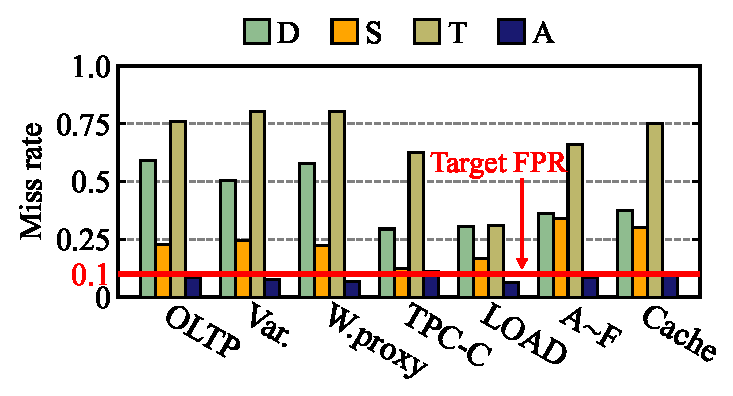
\includegraphics[width=\textwidth]{exp/miss_ratio/final-miss-ratio.eps}
            \vspace{-7pt}
   	        \caption{\FIXME{Miss ratio}} 
            \label{fig:miss-ratio}
    \end{minipage}
	\begin{minipage}[c]{0.71\textwidth}
        \begin{subfigure}[b]{0.64\textwidth}
            \centering
            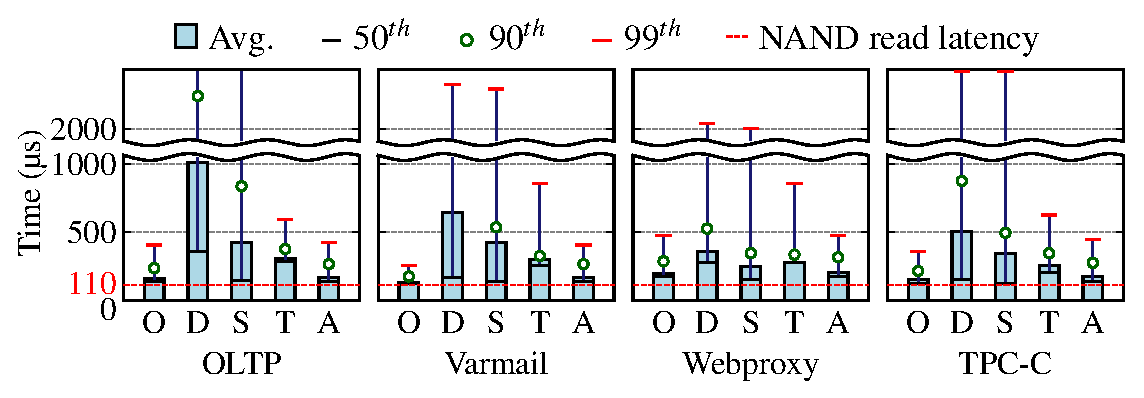
\includegraphics[width=\textwidth]{exp/filesystem/fs-latency.eps}
            \vspace{-10pt}
   	        \caption{\FIXME{Read latency}} 
            \label{fig:swap-latency}
        \end{subfigure}
        \begin{subfigure}[b]{0.345\textwidth}
            \centering
            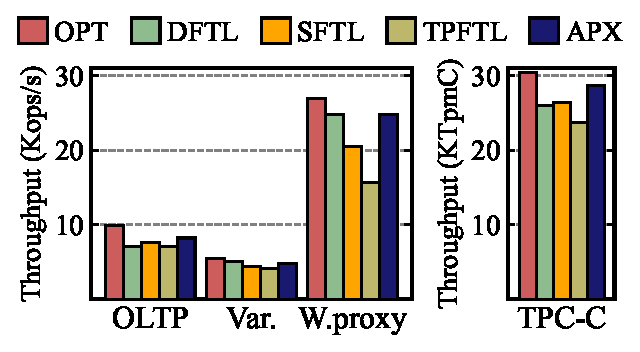
\includegraphics[width=\textwidth]{exp/filesystem/new-fs-throughput.eps}
            \vspace{0pt}
            \caption{Throughput} 
            \label{fig:swap-throughput}
        \end{subfigure}
        \vspace{-10pt}
	    \caption{Experimental results of Filebench and TPC-C}
	    \label{fig:exp-swap}
	\end{minipage}
\end{figure*}
\end{comment}

\begin{comment}
\begin{figure}[t]
\centering
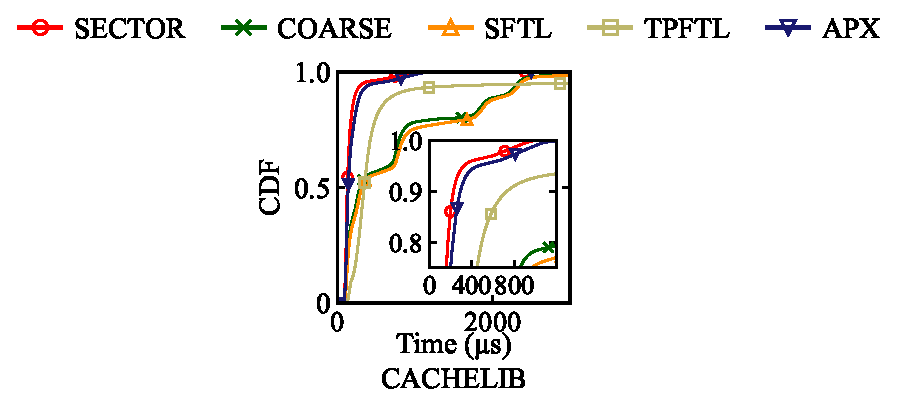
\includegraphics[width=0.8\linewidth]{exp/cache/CACHE_cdf.eps}
%\vspace{-3pt}
\caption{\FIXME{Latency of cache}}
\label{fig:cache-latency}
\end{figure}

\begin{figure}[t]
\centering
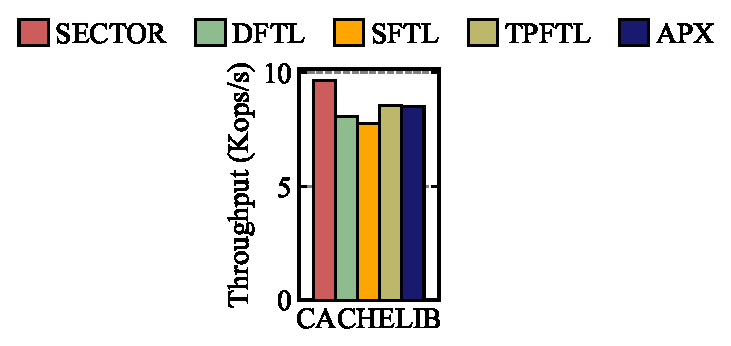
\includegraphics[width=0.8\linewidth]{exp/cache/CACHE_throughput.eps}
%\vspace{-3pt}
\caption{\FIXME{Throughput of cache}}
\label{fig:cache-throughput}
\end{figure}
\end{comment}

\begin{comment}

\begin{figure*}[t]
\centering
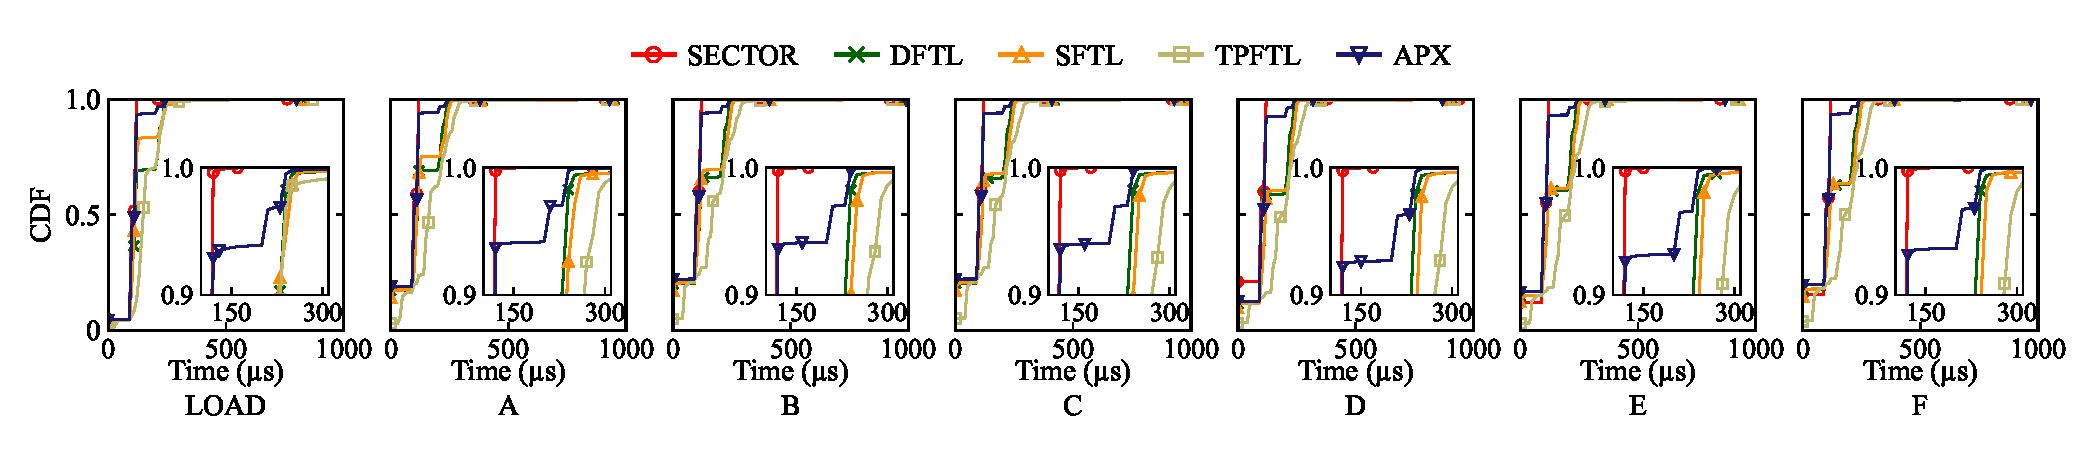
\includegraphics[width=\linewidth]{exp/swap/SWAP_cdf.eps}
%\vspace{-3pt}
\caption{\FIXME{CDF of read latency of YCSB benchmark}}
\label{fig:95swap-minmax}
\end{figure*}

\begin{figure*}[t]
\centering
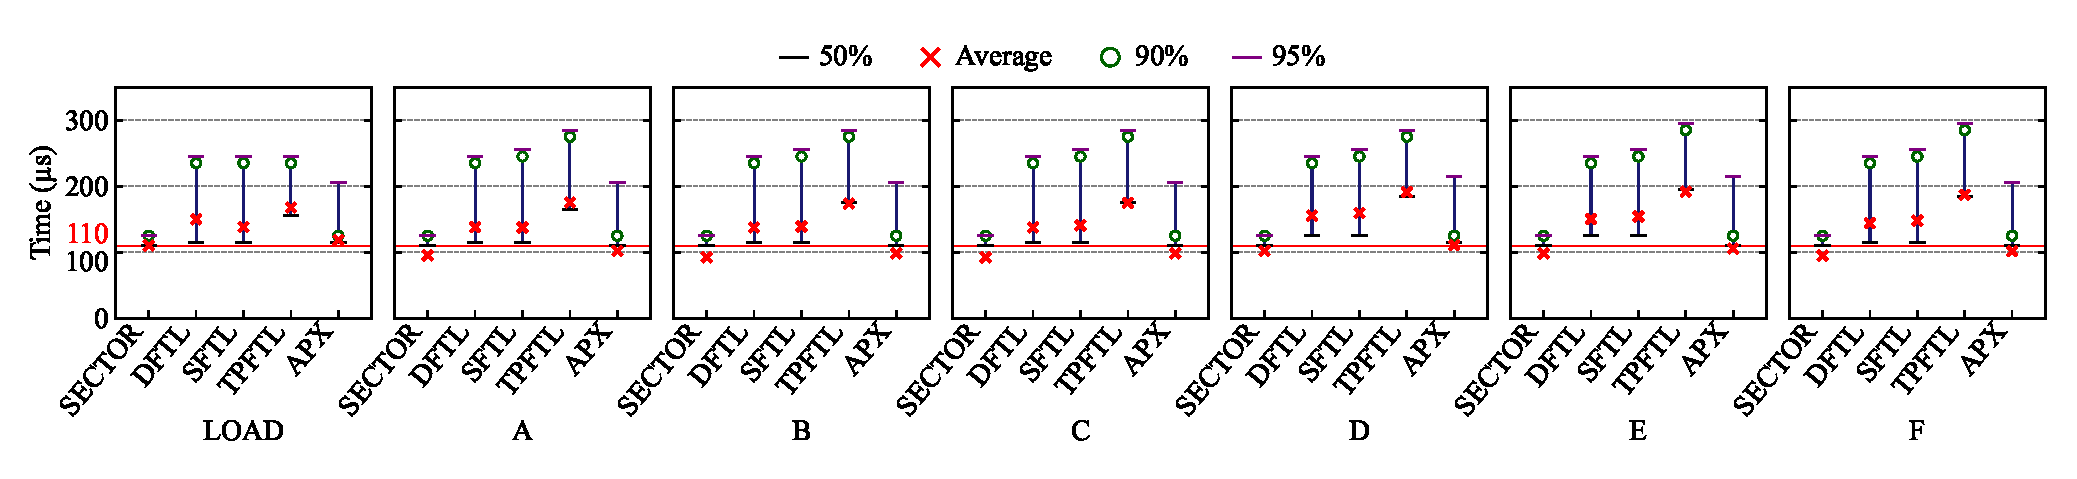
\includegraphics[width=\linewidth]{exp/swap/95_SWAP_minmax.eps}
%\vspace{-3pt}
\caption{\FIXME{Latency of YCSB benchmark (95\%)}}
\label{fig:99swap-minmax}
\end{figure*}


\begin{figure}[t]
\centering
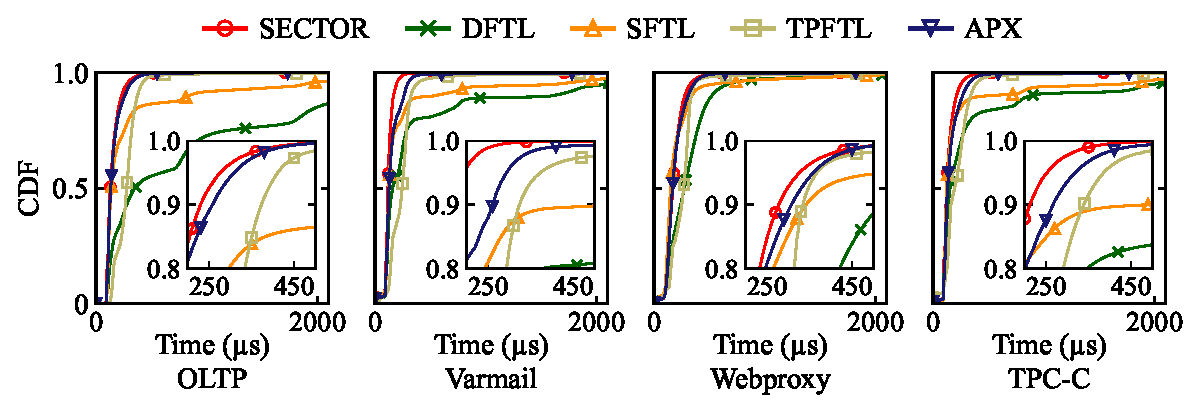
\includegraphics[width=\linewidth]{exp/filesystem/FS_cdf.eps}
%\vspace{-3pt}
\caption{\FIXME{CDF of read latency of Filebench and TPC-C}}
\label{fig:95fs-minmax}
\end{figure}

\begin{figure}[t]
\centering
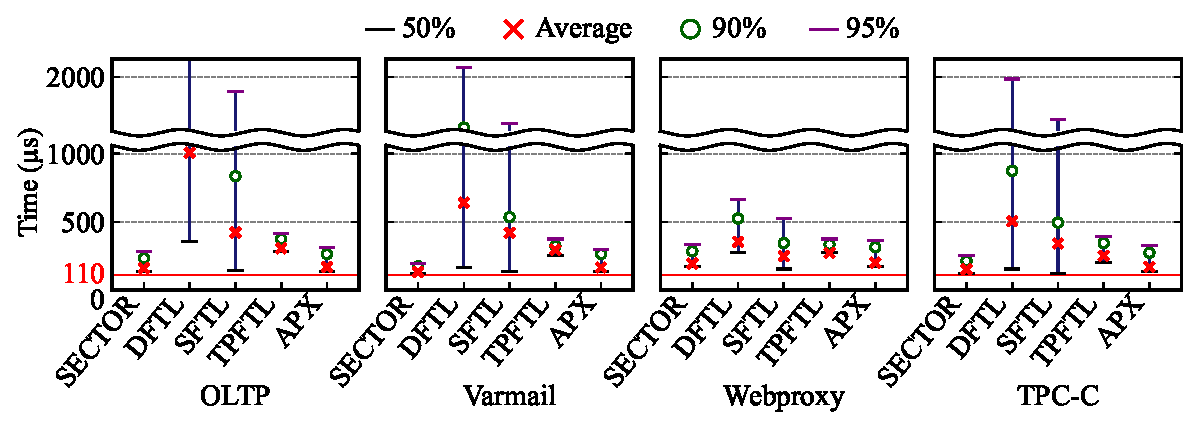
\includegraphics[width=\linewidth]{exp/filesystem/95_FS_minmax_brok.eps}
%\vspace{-3pt}
\caption{\FIXME{Latency of Filebench and TPC-C (95\%)}}
\label{fig:99fs-minmax}
\end{figure}

\begin{figure}[t]
\centering
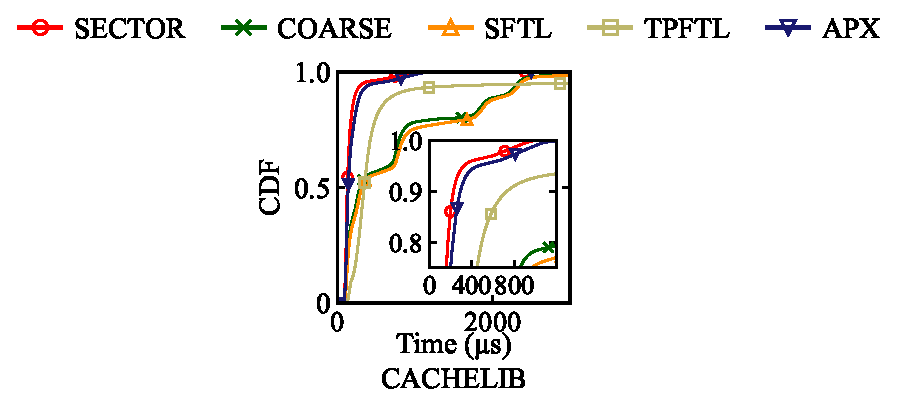
\includegraphics[width=0.8\linewidth]{exp/cache/CACHE_cdf.eps}
%\vspace{-3pt}
\caption{\FIXME{CDF of read latency of Cache system}}
\label{fig:99cache-minmax}
\end{figure}

\begin{figure}[t]
\centering
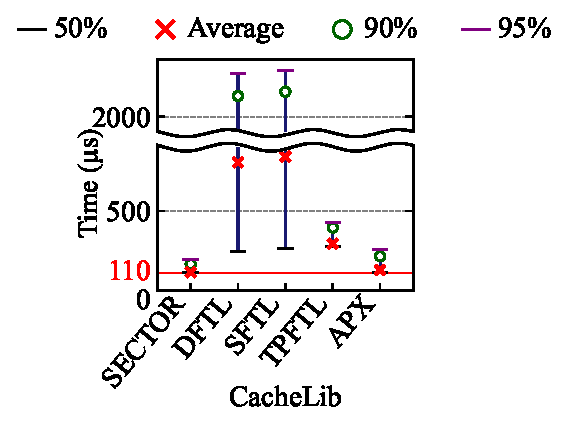
\includegraphics[width=0.6\linewidth]{exp/cache/95_CACHE_minmax_brok.eps}
%\vspace{-3pt}
\caption{\FIXME{Latency of Cache system (95\%)}}
\label{fig:95cache-minmax}
\end{figure}
\end{comment}


% \begin{figure*}[t]
%     %\vspace{0pt}
% 	\begin{minipage}[c]{0.675\textwidth}
% 	\centering
% 	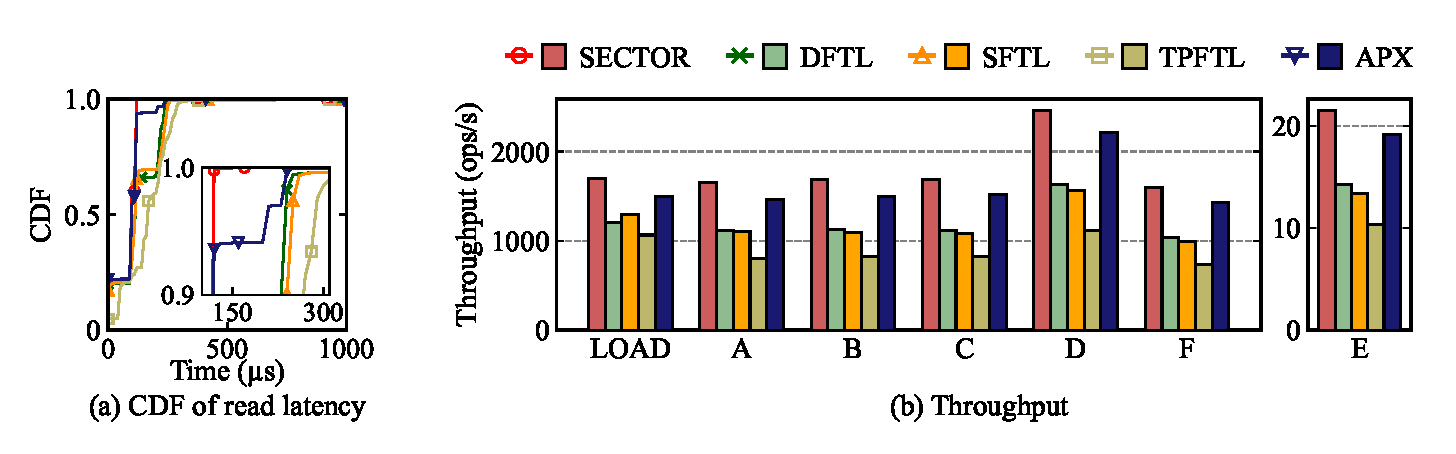
\includegraphics[width=\linewidth]{exp/filesystem/SWAP_cdf_throughput.eps}
%   	\caption{Performance of YCSB benchmark} 
% 	\label{fig:miss-ratio}
% 	\end{minipage}
% 	\begin{minipage}[c]{0.315\textwidth}
% 	\centering
% 	\vspace{11pt}
% 	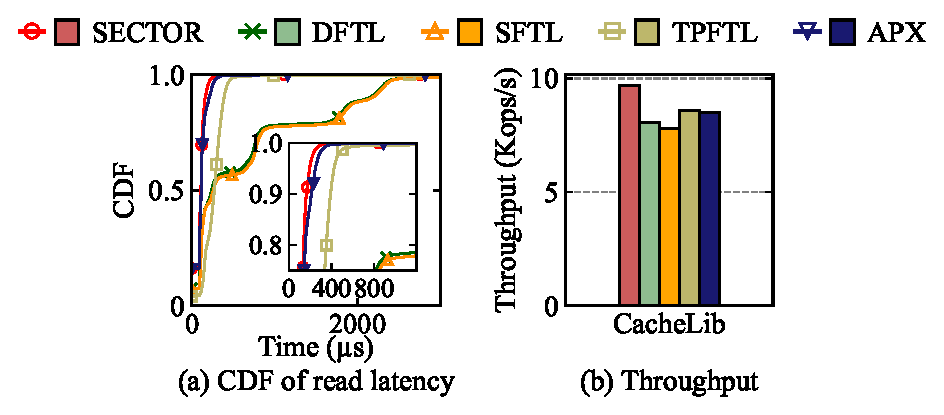
\includegraphics[origin=c,width=\linewidth]{exp/cache/CACHE_inter.eps}
%     \caption{Performance of CacheLib} 
% 	\label{fig:db-throughput}
%     \end{minipage}
% \end{figure*}

% \begin{figure*}[!t]
%     \centering
%     \begin{subfigure}[b]{0.57\textwidth}
%         \centering
%         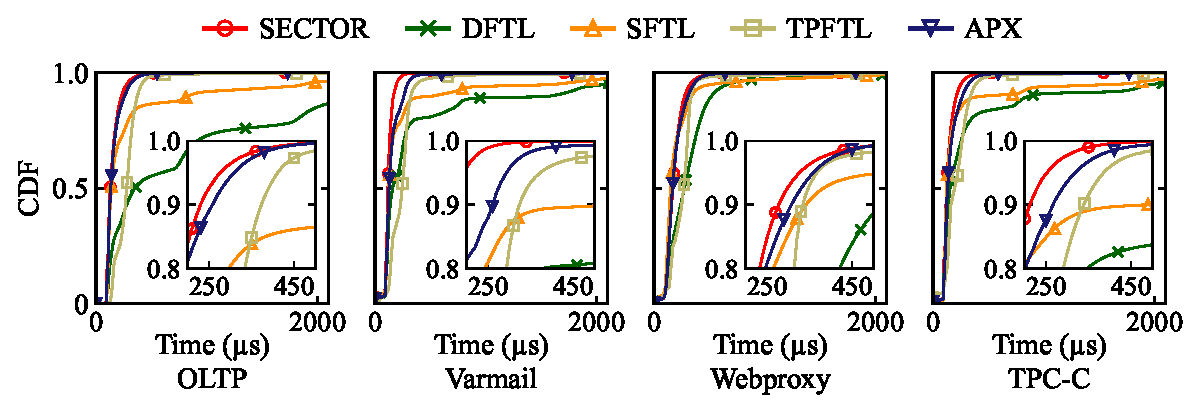
\includegraphics[width=\textwidth]{exp/filesystem/FS_cdf.eps}
%   	    \caption{CDF of read latency} 
%         \label{fig:filebench-latency}
%     \end{subfigure}
%     \begin{subfigure}[b]{0.356\textwidth}
%         \centering
%         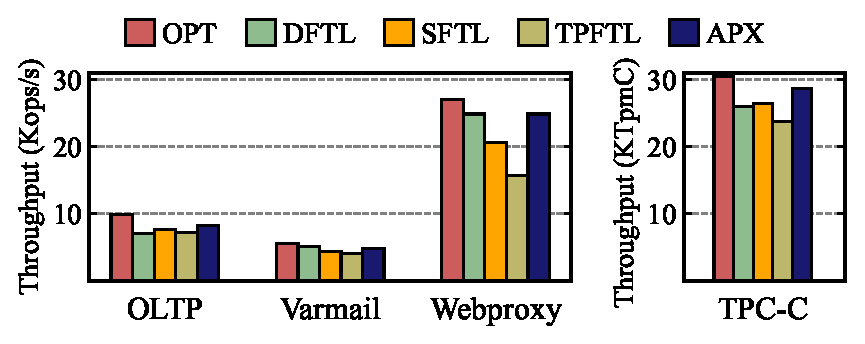
\includegraphics[width=\textwidth]{exp/filesystem/FS_throughput.eps}
%         \vspace{1pt}
%         \caption{Throughput} 
%         \label{fig:filebench-throughput}
%         \end{subfigure}
%     \vspace{-7pt}
% 	\caption{Experimental results of Filebench and TPC-C}
% 	\label{fig:filebench-results}
% \end{figure*}
